\begin{figure}[!htbp]
\centering
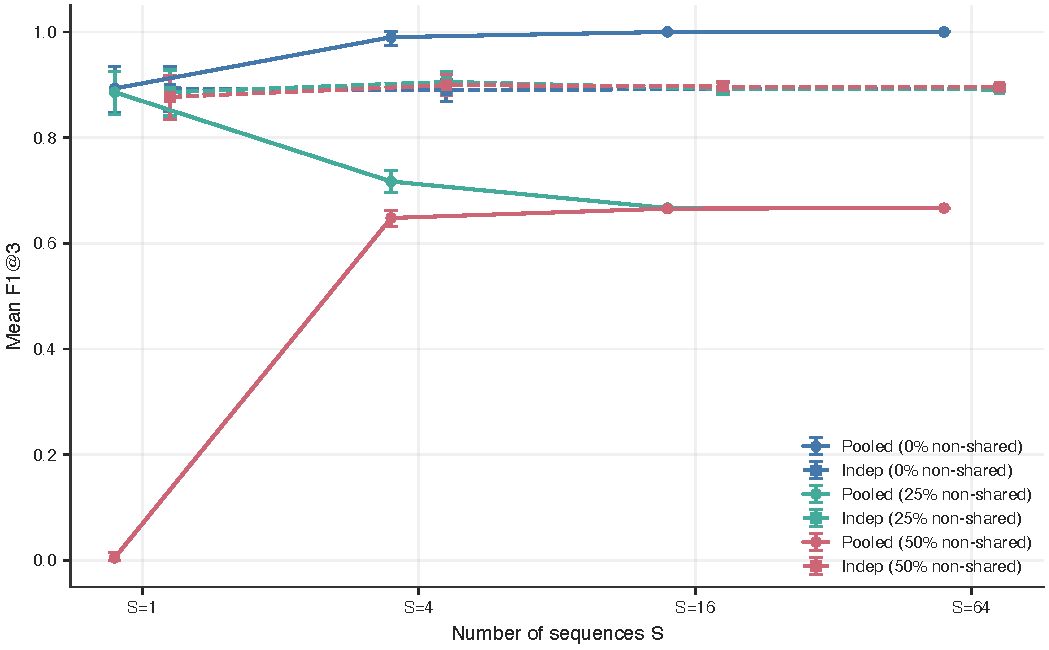
\includegraphics[width=0.92\linewidth]{figures/fig_E04_pooled.pdf}
\caption{Pooled versus independent boundary recovery across number of shared sequences
$S\in\{1,4,16,64\}$ and nonshared fraction $f\in\{0,0.25,0.5\}$.
Pooled F1@3 (solid) and independent per-sequence F1@3 (dashed), with 95\% bootstrap bands.
At full sharing ($f=0$), pooled F1 reaches 1.00 for $S\geq16$ while independent F1 remains
near 0.89 across all $S$. Under partial or complete nonsharing, pooled inference is
misspecified and pooled F1 degrades; independent inference is not affected.
F1 is evaluated against the common template boundaries for the pooled method
and against per-sequence actual boundaries for the independent method.}
\label{fig:planned-pooled-paper}
\end{figure}
